

%----------------------------------------------------------------------------------------
%	CHAPTER 1
%----------------------------------------------------------------------------------------
\chapter{Core}

In the following we wish to demonstrate hepstores core abilities with
short, simple examples. It is the aim to introduce the command line
functionality, which should give the user a clear guidance on how to
perform simple analyses. All arguments can be viewed via
%
\begin{changemargin}{1.5cm}{1.5cm} 
  \begin{lstlisting}[language=Bash]
    
    hepstore-module -h
  \end{lstlisting}
\end{changemargin}
%
In addition, there is the possibility to use hepstores modules from
within Pyhton, of course. In the appendix we collect the python
scripts needed to reproduce the plots presented in the
following. Furthermore, to support learning, these script contain one
level of complexity more in the sense, that we only show the
neccessary arguments in the following, while the scripts contain the
full information. All scripts can be found in the git repository at
'hepstore/documentation/examples/core'.


\section{Data}
The data we wish to use in the following is divided in two subsets for
classification, which one might call signal and background. The
feature (phase) space is two dimensional and has no units. The
background $B$ is gaussian with zero mean and a diagonal covariance
matrix of width three. The signal however, is composed of two
gaussians, $S_1$ and $S_2$. Mean and covariance ar quoted in the
following.
%
\begin{alignat}{3}
  \mu_{B}          &= \begin{bmatrix} 0.0 & 0.0 \end{bmatrix} &\qquad
  \text{cov}_{B}   &= \begin{bmatrix} 3.0 & 0.0 \\ 0.0 & 3.0 \end{bmatrix} \notag\\
  \mu_{S,1}        &= \begin{bmatrix} 2.5 & -2.5 \end{bmatrix} &\qquad
  \text{cov}_{S,1} &= \begin{bmatrix} 1.0 & 0.0 \\ 0.0 & 1.0 \end{bmatrix} \notag\\
  \mu_{S,2}        &= \begin{bmatrix} -1.4 & 0.8 \end{bmatrix} &\qquad
  \text{cov}_{S,2} &= \begin{bmatrix} 0.02 & 1.2 \\ -1.7 & 0.01 \end{bmatrix}
\end{alignat}
%




\section{Plotter}


produce some data
%
\begin{changemargin}{1.5cm}{1.5cm} 
  \lstinputlisting[numbers=left,firstnumber=1,firstline=1]{../examples/hepstore_plot/produce_data.py}
\end{changemargin}
%
plot with hepstore-plot
%
\begin{changemargin}{1.5cm}{1.5cm} 
  \lstinputlisting[numbers=left,firstnumber=1,firstline=1,language=Bash]{../examples/hepstore_plot/example.sh}
\end{changemargin}
%
%
show plots
%
\begin{figure}
  \centering
  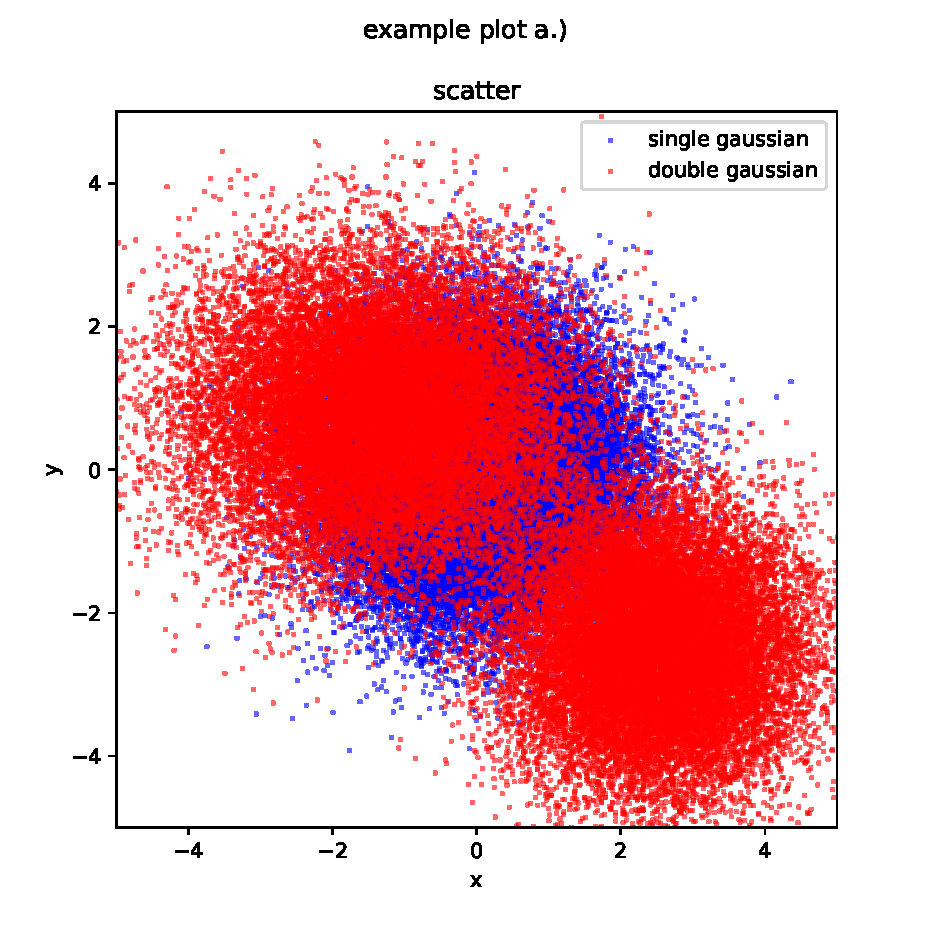
\includegraphics[width=0.3\textwidth]{../examples/hepstore_plot/example_a.pdf}
  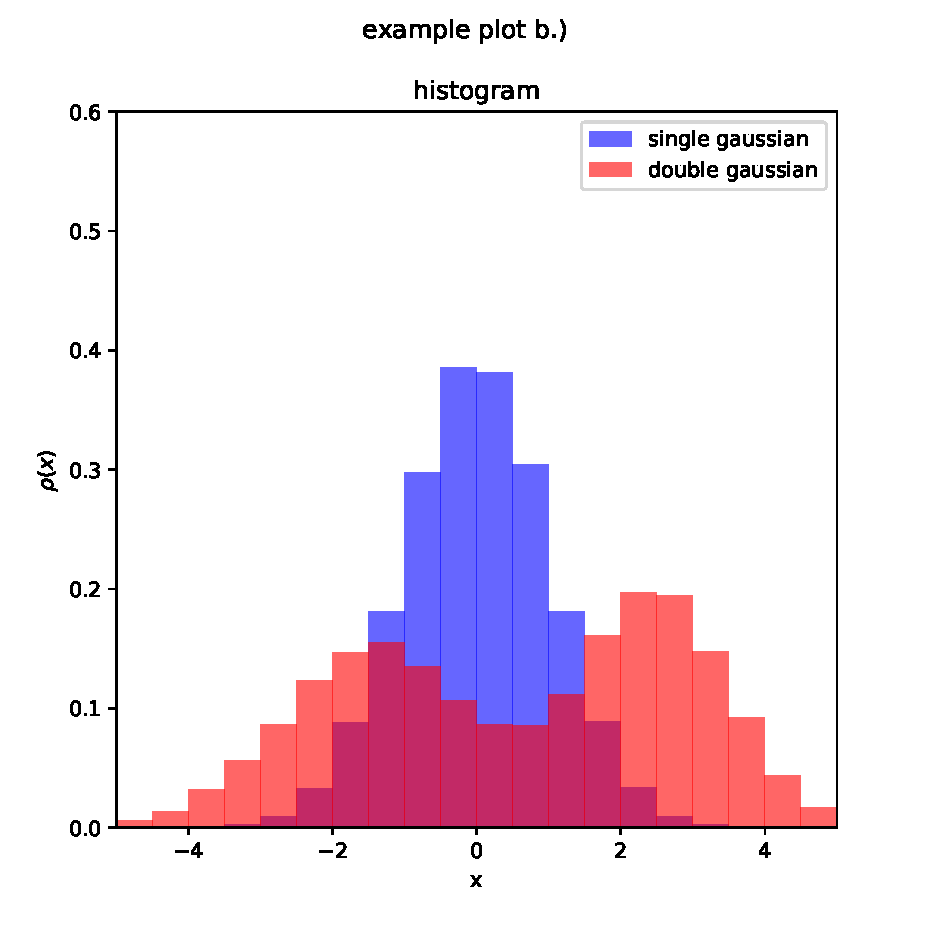
\includegraphics[width=0.3\textwidth]{../examples/hepstore_plot/example_b.pdf}
  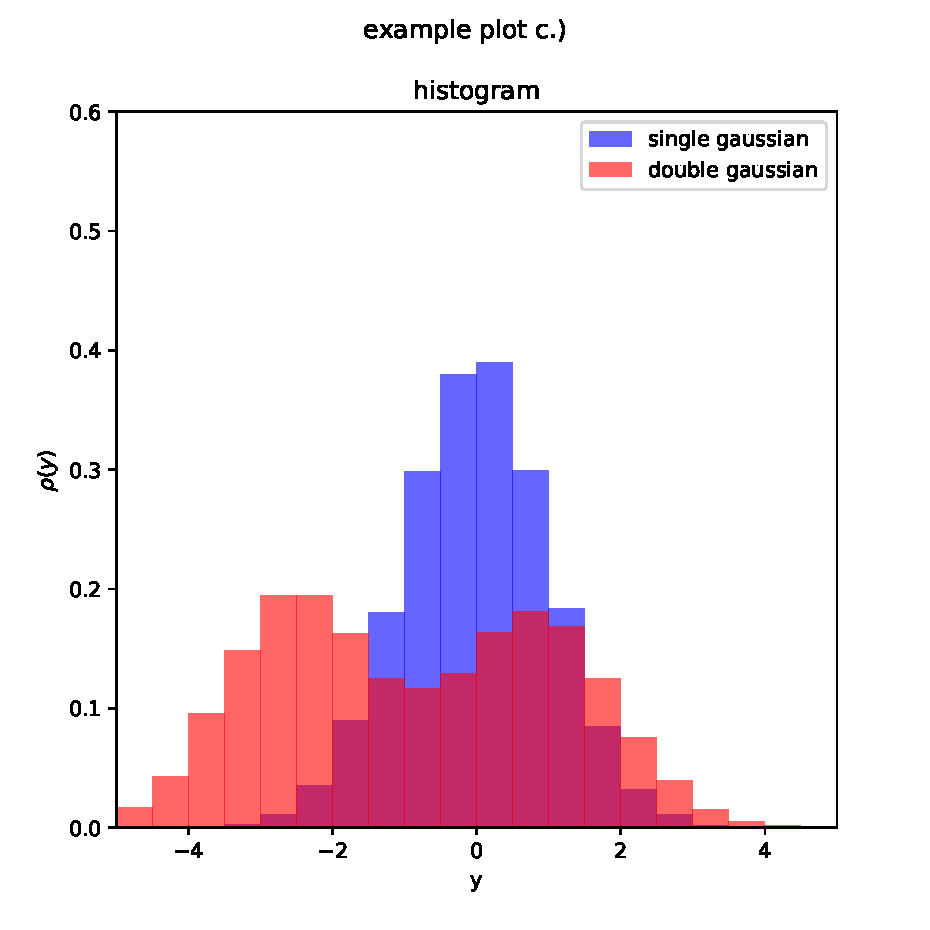
\includegraphics[width=0.3\textwidth]{../examples/hepstore_plot/example_c.pdf}
  \caption{}
  \label{fig:example_plotting}
\end{figure}
%


\section{School}

\subsection{Tuning}
The following Phyton script generates a set of pseudo data to which we
tune a Quadratic Discriminant Analysis (QDA) for classification
purposes.
%
\begin{changemargin}{1.5cm}{1.5cm} 
  \lstinputlisting[numbers=left,firstnumber=1,firstline=1]{../examples/core/school/tuning.py}
\end{changemargin}
%
%
\begin{figure}
  \centering
  \includegraphics[width=0.32\textwidth]{../examples/core/school/cross_validation.pdf}
  \includegraphics[width=0.32\textwidth]{../examples/core/school/learning_curve.pdf}
  \caption{}
  \label{fig:example_tuning}
\end{figure}
%
In Fig.~\ref{fig:example_tuning} we show, from left to right, the
parameter cross validation and the learning curve. We observe stable
and convergent behaviour.
%
\begin{table}[h!]
  \centering
  \begin{tabular}{c|c}
    parameter & value \\
    \hline \hline
    tol       & $2.64\times10^{-9}$ \\
    reg\_param& $1.18\times10^{-2}$\\
    \hline
    \end{tabular}
  \caption{}
  \label{tab:example_tuning}
\end{table}
%
The best tune parameter values are presented in
Tab.~\ref{tab:example_tuning}.

\subsection{Training}
The following Phyton script trains the previously tuned QDA on the
same training data set.
%
\begin{changemargin}{1.5cm}{1.5cm} 
  \lstinputlisting[numbers=left,firstnumber=1,firstline=1]{../examples/core/school/learning.py}
\end{changemargin}
%
%
\begin{figure}
  \centering
  \includegraphics[width=0.32\textwidth]{../examples/core/school/probability_map.pdf}
  \includegraphics[width=0.32\textwidth]{../examples/core/school/classifier_output.pdf}
  \includegraphics[width=0.32\textwidth]{../examples/core/school/roc.pdf}
  \caption{}
  \label{fig:example_training}
\end{figure}
%
In Fig.~\ref{fig:example_tuning} we display the training and testing
results. From the classifier output distribution we deduce that, as
expected, no over training occured. Furthermore, the probability map
shows that the classifier nicely maps the background shape. The ROC
curve diplayed may be used as input for statistical analysis.

\subsection{Working}

The following Phyton script generates a second set of data. The
distributions are the same. However, we changed the random
seed. Therefore, we assume in the following that the model models the
data correctly. We then let the trained classifier compute the
classification probability for the data.
%
\begin{changemargin}{1.5cm}{1.5cm} 
  \lstinputlisting[numbers=left,firstnumber=1,firstline=1]{../examples/core/school/working.py}
\end{changemargin}
%
%
\begin{figure}
  \centering
  \includegraphics[width=0.32\textwidth]{../examples/core/school/blind_distribution.pdf}
  \caption{}
  \label{fig:example_working}
\end{figure}
%
In Fig.~\ref{fig:example_working} we present the classifier output
distribution as computed from the new data set without labels. As can
be seen from the first bin there where about 500 signal events in the
sample.


\section{Statistics}

In general, one can perform statisticla analyses once the pdf's for
all processes are known. In addition, ROC curves contain all the
information needed to perform certain statistical analyses. In the
following we use the results produced with hepstore-school to compute
statistical quantities.

\subsection{Fit a Signal}
We like to estimate the number of signal and background events
contained in the joined data set data\_3.npy and data\_4.npy. As pdf
we use the trained and labeled classifier output distribution,
computed in Sec.~\ref{sec:}. As data the blinded distribution from
Sec.~\ref{sec:}.
%
\begin{changemargin}{1.5cm}{1.5cm} 
  \begin{lstlisting}[language=Bash]
    
    hepstore-statistics --fit --data blinded.npy --pdf cls_pdf_background.npy cls_pdf_signal.npy
  \end{lstlisting}
\end{changemargin}
%
We find $9974.5$ background events and $503.2$ signal events, whereas
the true value was $10000$ respectively $500$.

\subsection{Upper Bound on Signal Cross Section}
Next let us use the ROC curve from Sec.~\ref{sec:} to compute the
upper limit on a possible signal cross section. 
%
\begin{changemargin}{1.5cm}{1.5cm} 
  \begin{lstlisting}[language=Bash]
    
    hepstore-statistics --limit --roc roc.npy --xsec_b 10.0 --luminosity 100.0
  \end{lstlisting}
\end{changemargin}
%
Assuming a luminosity $\mathcal{L} = 100$ and a background cross
section of $\sigma_B = 10$, we compute an upper limit on the signal
cross section of $\sigma_s \le 0.131$. We use the ROC curve obtained
in the previous section. The optimal working point is at $\epsilon_S =
39\%$, corresponding to $\epsilon_B = 0.0014$.

\subsection{Poissonian Significance}
For given expected signal and background number of events we can
compute the expected Poissonian significance as function of the
classifier output.
%
\begin{changemargin}{1.5cm}{1.5cm} 
  \begin{lstlisting}[language=Bash]
    
    hepstore-statistics --significance --cls_b cls_pdf_background.npy --cls_s cls_pdf_signal.npy --xsec_s 0.5 --xsec_b 10. --luminosity 100.
  \end{lstlisting}
\end{changemargin}
%
%
\begin{figure}
  \centering
  \includegraphics[width=0.32\textwidth]{../examples/core/statistic/significance.pdf}
  \caption{}
  \label{fig:example_statistic}
\end{figure}
%
In Fig.~\ref{fig:example_statistic} we present the classifier output
cut dependent significance. Furthermore, we show the corresponding
signal and background efficiencies, $\epsilon_S$ and $\epsilon_B$.XS

%\subsection{Significance from Loglikelihood}



\section{Physics}

\subsection{Particles}
Let us use the same data set as above. We interpret the $(x,y)$
distribution to be the $(p_x,p_y)$ steming from particles with a comen
origin in direction. The background we identify as jets and the signal
as electrons. Let us further assume that the have different production
energies, which in addition are smeared by gaussian noise.
%
\begin{figure}
  \centering
  \includegraphics[width=0.32\textwidth]{../examples/core/physics/mass.pdf}
  \caption{}
  \label{fig:example_physics}
\end{figure}
%
In Fig.~\ref{fig:example_physics} we present the invariant mass
distribution for every unique pairing of jets respectively electrons.



%----------------------------------------------------------------------------------------
%	CHAPTER 2
%----------------------------------------------------------------------------------------
\chapter{Framework}

\section{Collider}



\section{Corsika}
\section{Herwig}
\section{Comparison}
\section{Reproducibility Script}


\subsection{List}
'hepstore-eas -L'

As this is a specific air shower framework we organise everything with
respect to the following scheme: energy -> primary particle ->
physical process -> MC generator -> nucleon model -> final state the
-{}-list argument searches for this structure and lists the following
possible contents hard events -> attempted showers -> showeres ->
observables

\subsection{Generation}

'hepstore-eas -G'

we interface from the hepstore.docker family (more details in
appendix) and provide automated runcards for herwig to produce events
which may be showerd by corsika

\subsubsection{Nucleon Modle}

we provide two nucleon models 'full' and 'fragmented'

\subsection{Shower}

'hepstore-eas -S'

we interface from the hepstore.docker family and provide automated
runcards for corsika to either shower events generted with '-G' or
produce corsika stand alone showers (internal corsika di-jet
production) when using '-C 7.4' (here 7.4 is the version vor the
docker image)

\subsection{Observables}

'hepstore-eas -A'

we provide our own event class to read corsika produced extended air
showers. inspired by rivet we allow for dynamic load of user analysis
modules and provide one example for such, constructing $\rho_\mu$ and
$X_\text{max}$. hepstore-eas automatically provides its output in .npy
format


%----------------------------------------------------------------------------------------
%	CHAPTER 2
%----------------------------------------------------------------------------------------
\chapter{Analysis}

\section{Sandbox}



\section{Arxiv}


\section{Published}


%----------------------------------------------------------------------------------------
%	CHAPTER 3
%----------------------------------------------------------------------------------------
\chapter{Example Scripts}

\section{Core}
~\\
\subsection{Data}
~\\
%
\begin{changemargin}{1.5cm}{1.5cm} 
  \lstinputlisting[numbers=left,firstnumber=1,firstline=1]{../examples/core/data/produce_data.py}
\end{changemargin}
%

\subsection{Plotter}
~\\
%
\begin{changemargin}{1.5cm}{1.5cm} 
  \lstinputlisting[numbers=left,firstnumber=1,firstline=1]{../examples/core/plotter/example.py}
\end{changemargin}
%

\subsection{School}
~\\
\subsubsection{Tuning}
~\\
%
\begin{changemargin}{1.5cm}{1.5cm} 
  \lstinputlisting[numbers=left,firstnumber=1,firstline=1]{../examples/core/school/tuning.py}
\end{changemargin}
%

\subsubsection{Learning}
~\\
%
\begin{changemargin}{1.5cm}{1.5cm} 
  \lstinputlisting[numbers=left,firstnumber=1,firstline=1]{../examples/core/school/learning.py}
\end{changemargin}
%

\subsubsection{Working}
~\\
%
\begin{changemargin}{1.5cm}{1.5cm} 
  \lstinputlisting[numbers=left,firstnumber=1,firstline=1]{../examples/core/school/working.py}
\end{changemargin}
%

\subsection{Statistics}
~\\
\subsubsection{Fit}
~\\
%
\begin{changemargin}{1.5cm}{1.5cm} 
  \lstinputlisting[numbers=left,firstnumber=1,firstline=1]{../examples/core/statistic/fit.py}
\end{changemargin}
%

\subsubsection{Limit}
~\\
%
\begin{changemargin}{1.5cm}{1.5cm} 
  \lstinputlisting[numbers=left,firstnumber=1,firstline=1]{../examples/core/statistic/upper_bound.py}
\end{changemargin}
%

\subsubsection{significance}
~\\
%
\begin{changemargin}{1.5cm}{1.5cm} 
  \lstinputlisting[numbers=left,firstnumber=1,firstline=1]{../examples/core/statistic/significance.py}
\end{changemargin}
%
\section{Physics}
\subsubsection{Particles}
~\\
%
\begin{changemargin}{1.5cm}{1.5cm} 
  \lstinputlisting[numbers=left,firstnumber=1,firstline=1]{../examples/core/physics/particles.py}
\end{changemargin}
%

\section{Framework}

\section{Analysis}
\subsection{Sandbox}
\subsubsection{Cosmic Rays}

